\documentclass[aspectratio=169, xcolor=dvipsnames]{beamer}

% --- Theme Setup ---
\usetheme{Madrid}
\usecolortheme{default}

% --- Packages ---
\usepackage{graphicx}
\usepackage{xcolor}
\usepackage{booktabs}
\usepackage{hyperref}
\usepackage{adjustbox}
\usepackage{amssymb}
\usepackage{longtable}
\usepackage{caption}
\usepackage{tikz}
\usetikzlibrary{mindmap,trees,shadows,arrows.meta,positioning,shapes.geometric,calc,chains}

% --- Title Information ---
\title{Module 05}
\subtitle{Introduction to DBMS/2}
\author{Milav Dabgar}
\institute{www.milav.in}
\date{\today}

\begin{document}

% Title Slide
\begin{frame}
    \titlepage
\end{frame}

\begin{frame}{Module Recap}
    \begin{itemize}
        \item Basic notions and terminology of database management systems
        \item Role of data models and languages
        \item Approaches to database design
    \end{itemize}
\end{frame}

\begin{frame}{Module Objectives}
    \begin{itemize}
        \item To understand models of database management systems
        \item To familiarize with major components of a database engine
        \item To familiarize with database internals and architecture
        \item To understand the historical perspective
    \end{itemize}
\end{frame}

\begin{frame}{Module Outline}
    \begin{itemize}[<+->]
        \item Database Design
        \item OO Relational Model
        \item XML
        \item Database Engine
        \begin{itemize}
            \item Storage Management
            \item Query Processing
            \item Transaction Management
        \end{itemize}
        \item Database Internals and Architecture
        \item Database Users and Administrators
    \end{itemize}
\end{frame}

\section{Database Design}

\begin{frame}
  \vfill
  \centering
  \begin{beamercolorbox}[sep=8pt,center,shadow=true,rounded=true]{title}
    \usebeamerfont{title}Database Design\par%
  \end{beamercolorbox}
  \vfill
\end{frame}

\begin{frame}{Database Design}
    \begin{block}{Defining the Structure}
        The process of designing the general structure of the database:
    \end{block}
    
    \uncover<2->{
        \begin{itemize}[<+->]
            \item \textbf{Logical Design} -- Deciding on the database schema. Database design requires that we find a good collection of relation schema
            \begin{itemize}
                \item \textbf{Business decision}: What attributes should we record in the database?
                \item \textbf{Computer Science decision}: What relation schemas should we have and how should the attributes be distributed among the various relation schemas?
            \end{itemize}
            \item \textbf{Physical Design} -- Deciding on the physical layout of the database
        \end{itemize}
    }
\end{frame}

\begin{frame}{Database Design (2)}
    \textbf{Is there any problem with this relation?}
    \vspace{0.5em}
    \begin{center}
        \begin{adjustbox}{max width=\textwidth}
        \begin{tabular}{|l|l|l|l|l|l|}
        \hline
        \textbf{ID} & \textbf{name} & \textbf{salary} & \textbf{dept\_name} & \textbf{building} & \textbf{budget} \\ \hline
        22222 & Einstein & 95000 & Physics & Watson & 70000 \\ \hline
        12121 & Wu & 90000 & Finance & Painter & 120000 \\ \hline
        32343 & El Said & 60000 & History & Painter & 50000 \\ \hline
        45565 & Katz & 75000 & Comp. Sci. & Taylor & 100000 \\ \hline
        98345 & Kim & 80000 & Elec. Eng. & Taylor & 85000 \\ \hline
        76766 & Crick & 72000 & Biology & Watson & 90000 \\ \hline
        10101 & Srinivasan & 65000 & Comp. Sci. & Taylor & 100000 \\ \hline
        58583 & Califieri & 62000 & History & Painter & 50000 \\ \hline
        83821 & Brandt & 92000 & Comp. Sci. & Taylor & 100000 \\ \hline
        15151 & Mozart & 40000 & Music & Packard & 80000 \\ \hline
        33456 & Gold & 87000 & Physics & Watson & 70000 \\ \hline
        76543 & Singh & 80000 & Finance & Painter & 120000 \\ \hline
        \end{tabular}
        \end{adjustbox}
    \end{center}
\end{frame}

\begin{frame}{Database Design (3)}
    \begin{columns}
        \begin{column}{0.5\textwidth}
            \textbf{(a) The instructor table}
            \begin{center}
                \begin{adjustbox}{max width=\textwidth}
                \begin{tabular}{|l|l|l|l|}
                \hline
                \textbf{ID} & \textbf{name} & \textbf{dept\_name} & \textbf{salary} \\ \hline
                22222 & Einstein & Physics & 95000 \\ \hline
                12121 & Wu & Finance & 90000 \\ \hline
                32343 & El Said & History & 60000 \\ \hline
                \dots & \dots & \dots & \dots \\ \hline
                \end{tabular}
                \end{adjustbox}
            \end{center}
        \end{column}
        \begin{column}{0.5\textwidth}
            \textbf{(b) The department table}
            \begin{center}
                \begin{adjustbox}{max width=\textwidth}
                \begin{tabular}{|l|l|l|}
                \hline
                \textbf{dept\_name} & \textbf{building} & \textbf{budget} \\ \hline
                Comp. Sci. & Taylor & 100000 \\ \hline
                Biology & Watson & 90000 \\ \hline
                Elec. Eng. & Taylor & 85000 \\ \hline
                Music & Packard & 80000 \\ \hline
                Finance & Painter & 120000 \\ \hline
                History & Painter & 50000 \\ \hline
                Physics & Watson & 70000 \\ \hline
                \end{tabular}
                \end{adjustbox}
            \end{center}
        \end{column}
    \end{columns}
\end{frame}

\begin{frame}{Design Approaches}
    Need to come up with a methodology to ensure that each relations in the database is good. Two ways of doing so:
    
    \uncover<2->{
        \begin{exampleblock}{Methodologies}
            \begin{itemize}[<+->]
                \item \textbf{Entity Relationship Model} (Chapter 7)
                \begin{itemize}
                    \item[$\triangleright$] Models an enterprise as a collection of entities and relationships
                    \item[$\triangleright$] Represented diagrammatically by an entity-relationship diagram
                \end{itemize}
                \item \textbf{Normalization Theory} (Chapter 8)
                \begin{itemize}
                    \item[$\triangleright$] Formalize what designs are bad, and test for them
                \end{itemize}
            \end{itemize}
        \end{exampleblock}
    }
\end{frame}

\section{Object-Relational Data Models}

\begin{frame}
  \vfill
  \centering
  \begin{beamercolorbox}[sep=8pt,center,shadow=true,rounded=true]{title}
    \usebeamerfont{title}Object-Relational Data Models\par%
  \end{beamercolorbox}
  \vfill
\end{frame}

\begin{frame}{Object-Relational Data Models}
    \begin{alertblock}{Limitations of Relational Model}
        Relational model explicitly limits storage to flat, atomic values.
    \end{alertblock}
    
    \uncover<2->{
        \begin{block}{Object Relational Extensions}
            \begin{itemize}[<+->]
                \item Extend the relational data model by including object orientation and constructs to deal with added data types
                \item Allow attributes of tuples to have complex types, including non-atomic values such as nested relations
                \item Preserve relational foundations, in particular the declarative access to data, while extending modeling power
                \item Provide upward compatibility with existing relational languages
            \end{itemize}
        \end{block}
    }
\end{frame}

\section{XML: Extensible Markup Language}

\begin{frame}
  \vfill
  \centering
  \begin{beamercolorbox}[sep=8pt,center,shadow=true,rounded=true]{title}
    \usebeamerfont{title}XML: Extensible Markup Language\par%
  \end{beamercolorbox}
  \vfill
\end{frame}

\begin{frame}{XML: Extensible Markup Language}
    \begin{itemize}[<+->]
        \item Defined by the WWW Consortium (W3C)
        \item Originally intended as a document markup language not a database language
        \item The ability to specify new tags, and to create nested tag structures made XML a great way to exchange data, not just documents
        \item XML has \textbf{become the basis} for all new generation data interchange formats
        \item A wide variety of tools is available for parsing, browsing and querying XML documents/data
    \end{itemize}
\end{frame}

\section{Database Engine}

\begin{frame}
  \vfill
  \centering
  \begin{beamercolorbox}[sep=8pt,center,shadow=true,rounded=true]{title}
    \usebeamerfont{title}Database Engine\par%
  \end{beamercolorbox}
  \vfill
\end{frame}

\begin{frame}{Database Engine}
    \begin{block}{Core Components}
        \begin{itemize}[<+->]
            \item Storage manager
            \item Query processing
            \item Transaction manager
        \end{itemize}
    \end{block}
\end{frame}

\begin{frame}{Storage Management}
    \begin{block}{The Storage Manager}
        A program module that provides the interface between the low-level data stored in the database and the application programs and queries submitted to the system.
    \end{block}
    
    \uncover<2->{
        \begin{itemize}[<+->]
            \item The storage manager is responsible for:
            \begin{itemize}
                \item Interaction with the OS file manager
                \item Efficient storing, retrieving and updating of data
            \end{itemize}
            \item Issues: Storage access, File organization, Indexing and hashing
        \end{itemize}
    }
\end{frame}

\begin{frame}{Query Processing}
    \begin{center}
        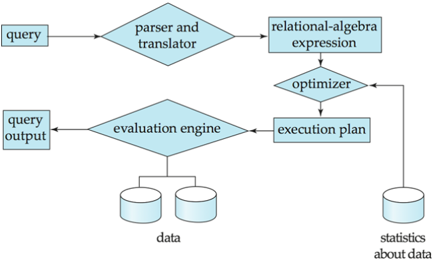
\includegraphics[height=0.7\textheight, width=0.9\textwidth, keepaspectratio]{../Lecture 1.5 - Intro to DBMS2_artifacts/image_000020_fac6872c7e5363b6930e02d55e3f1457a8b745b8ac581db16b57e237d2c739ab.png}
    \end{center}
\end{frame}

\begin{frame}{Query Processing (2)}
    \begin{itemize}[<+->]
        \item Alternative ways of evaluating a given query
        \begin{itemize}
            \item Equivalent expressions
            \item Different algorithms for each operation
        \end{itemize}
        \item \textbf{Cost difference} between a good and a bad way of evaluating a query can be enormous
        \item Need to estimate the cost of operations
        \begin{itemize}
            \item Depends critically on statistical information about relations which the database must maintain
            \item Need to estimate statistics for intermediate results to compute cost of complex expressions
        \end{itemize}
    \end{itemize}
\end{frame}

\begin{frame}{Transaction Management}
    \begin{alertblock}{Challenges}
        What if the system fails? What if more than one user is concurrently updating the same data?
    \end{alertblock}
    
    \uncover<2->{
        \begin{itemize}[<+->]
            \item A \textbf{transaction} is a collection of operations that performs a single logical function in a database application.
            \item \textbf{Transaction-management component} ensures that the database remains in a consistent (correct) state despite system failures and transaction failures.
            \item \textbf{Concurrency-control manager} controls the interaction among the concurrent transactions, to ensure the consistency of the database.
        \end{itemize}
    }
\end{frame}

\section{Database System Internals}

\begin{frame}
  \vfill
  \centering
  \begin{beamercolorbox}[sep=8pt,center,shadow=true,rounded=true]{title}
    \usebeamerfont{title}Database System Internals\par%
  \end{beamercolorbox}
  \vfill
\end{frame}

\begin{frame}{Database System Internals}
    \begin{center}
        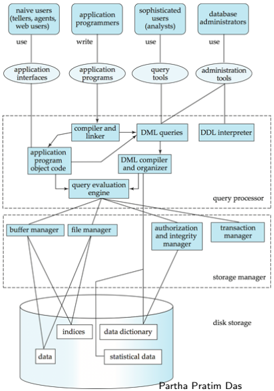
\includegraphics[height=0.8\textheight, width=0.9\textwidth, keepaspectratio]{../Lecture 1.5 - Intro to DBMS2_artifacts/image_000026_e32060a8c1581e858872251111aba5fd43c88883e445a382559ff7b6324c2bf2.png}
    \end{center}
\end{frame}

\begin{frame}{Database Architecture}
    The architecture of a database system is greatly influenced by the underlying computer system on which the database is running:
    
    \begin{itemize}
        \item Centralized
        \item Client-server
        \item Parallel (multi-processor)
        \item Distributed
        \item Cloud
    \end{itemize}
\end{frame}

\begin{frame}{Database Architecture (2)}
    \begin{center}
        
        \vspace{1em}
        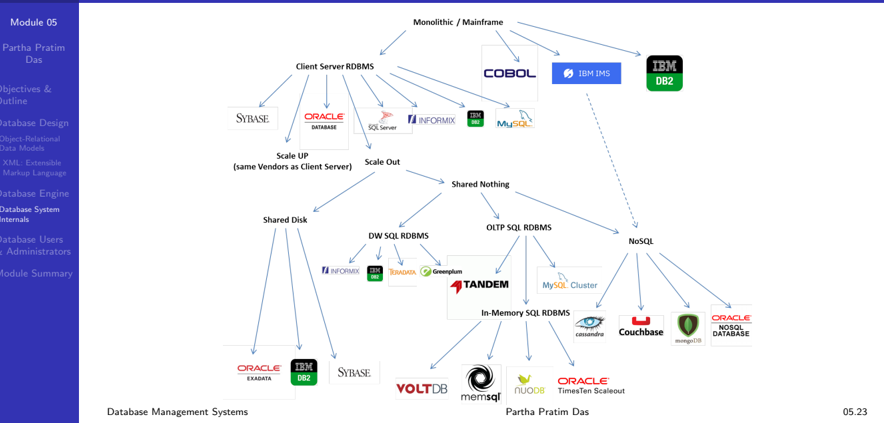
\includegraphics[height=0.4\textheight, width=0.9\textwidth, keepaspectratio]{../Lecture 1.5 - Intro to DBMS2_artifacts/image_000030_fa0f7d62a3c53dd9a7fe57674060e5275267add9a8147d764d446412fa046023.png}
    \end{center}
\end{frame}

\section{Database Users and Administrators}

\begin{frame}
  \vfill
  \centering
  \begin{beamercolorbox}[sep=8pt,center,shadow=true,rounded=true]{title}
    \usebeamerfont{title}Database Users and Administrators\par%
  \end{beamercolorbox}
  \vfill
\end{frame}

\begin{frame}{Database Users and Administrators}
    \begin{center}
    \end{center}
\end{frame}

\begin{frame}{Database Users and Administrators (2)}
    \begin{center}
        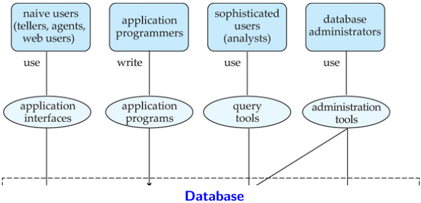
\includegraphics[height=0.8\textheight, width=0.9\textwidth, keepaspectratio]{../Lecture 1.5 - Intro to DBMS2_artifacts/image_000034_88e56afa27b8d786cef511364446b691aab94bda2e4aef8c93e328144a3984ae.png}
    \end{center}
\end{frame}

\begin{frame}{Module Summary}
    \begin{itemize}
        \item Introduced models of database management systems
        \item Familiarized with major components of a database engine
        \item Familiarized with database internals and architecture
    \end{itemize}
    
    \vspace{2em}
    \begin{center}
    \small \textit{Slides used in this presentation are borrowed from \url{http://db-book.com/} with kind permission of the authors.} \\
    \small \textit{Edited and new slides are marked with 'PPD'.}
    \end{center}
\end{frame}

\end{document}
